% Generated raster illustration, laid out with ordinary TeX boxes.
% Shared template placement remains unchanged to preserve the frozen cover.
\begin{frame}{Local vs Cooperative}
  \SlideBody{%
    \centering
    {\fontsize{12}{14}\selectfont\bfseries
      \makebox[4.8cm]{\textcolor{MoverCyan}{Vehicle A's LiDAR}}\hfill
      \makebox[4.8cm]{\textcolor[HTML]{D97920}{Vehicle B's LiDAR}}\hfill
      \makebox[4.8cm]{\textcolor{MoverDetailBlue}{Combined View}}\par}
    \vspace{0.12cm}
    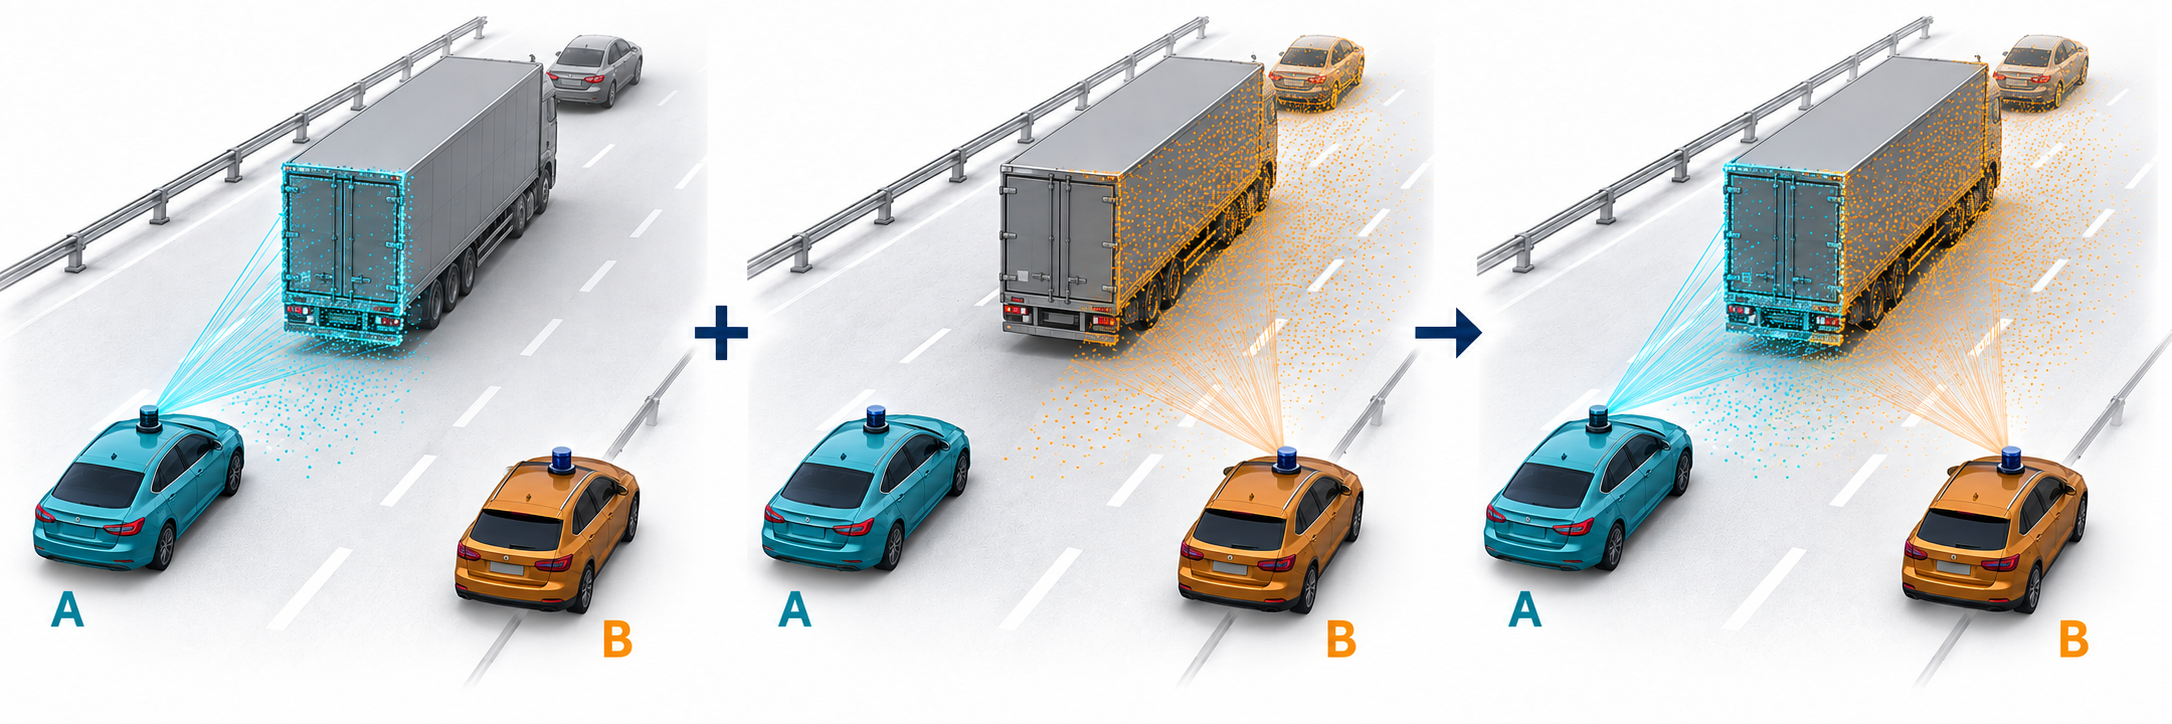
\includegraphics[width=14.8cm,height=4.70cm,keepaspectratio]{assets/illustrations/lidar-cooperation-v2.png}\par
    \vspace{0.04cm}
    {\fontsize{10.5}{12.8}\selectfont
      \makebox[4.8cm]{Truck Blocks A's View}\hfill
      \makebox[4.8cm]{B Sees the Hidden Car}\hfill
      \makebox[4.8cm]{Shared LiDAR Observations}\par}
  }
  \SlideSource{AI-generated illustration.}
\end{frame}
